\documentclass[conference]{IEEEtran}
\IEEEoverridecommandlockouts

\usepackage{cite}
\usepackage{amsmath,amssymb,amsfonts}
\usepackage{algorithmic}
\usepackage{graphicx}
\usepackage{textcomp}
\usepackage{xcolor}
\usepackage{booktabs}
\usepackage{multirow}
\usepackage{url}

% Tight IEEE float and spacing controls
\setlength{\textfloatsep}{5pt plus 1.0pt minus 1.5pt}
\setlength{\floatsep}{4pt plus 1.0pt minus 1.0pt}
\setlength{\intextsep}{4pt plus 1.0pt minus 1.0pt}
\setlength{\dbltextfloatsep}{6pt plus 1.0pt minus 1.5pt}
\setlength{\dblfloatsep}{5pt plus 1.0pt minus 1.0pt}

\def\BibTeX{{\rm B\kern-.05em{\sc i\kern-.025em b}\kern-.08em
    T\kern-.1667em\lower.7ex\hbox{E}\kern-.125emX}}

\begin{document}

\title{A Multi-Modal Edge-AI Framework for Real-Time Pediatric Safety Monitoring via Acoustic and Spatial-Temporal Vision Analytics}

\author{
\IEEEauthorblockN{K. V. U. De Abrew\IEEEauthorrefmark{1}, A. M. T. A. Samarakkody\IEEEauthorrefmark{1}, Pradeep K. W. Abeygunawardhana\IEEEauthorrefmark{1}, and Samitha Vidhanaarachchi\IEEEauthorrefmark{2}}
\IEEEauthorblockA{\IEEEauthorrefmark{1}\textit{Department of Information Technology, Faculty of Computing, Sri Lanka Institute of Information Technology, Malabe, Sri Lanka}\\
Email: \{vidushaupashaly, thivinasamarakkody\}@gmail.com, pradeep.a@sliit.lk}
\IEEEauthorblockA{\IEEEauthorrefmark{2}\textit{School of Information Technology, Murdoch University, Murdoch, Western Australia 6150, Australia}\\
Email: samitha.v@murdoch.edu.au}
}

\maketitle

\begin{abstract}
<<<<<<< Updated upstream
Single-sensor domestic child-safety monitors suffer from complementary blind spots and high false-alarm rates that cause acute caregiver alert fatigue. This paper presents a multi-modal edge-AI framework unifying acoustic and vision analytics into a synchronized, privacy-preserving threat evaluation engine. The acoustic subsystem deploys an ultra-low-power ESP32-S3 edge node streaming discrete 3.0-second audio frames over an isolated local WLAN to an on-premise gateway, where a lightweight 1D-CNN-LSTM classifier (AudioThreatNet, 97,602 parameters, 14.27 MFLOPs) captures non-linear vocal distress onset and pitch dynamics. To resolve alert fatigue caused by benign domestic vocalizations without compromising child safety, a 64-dimensional multi-band spectral-cepstral speaker embedding gate performs Cosine distance verification against enrolled caregiver templates, conditioned on a high-frequency pediatric scream band veto ($R_{\text{scream}} < 0.22$) and vision context. Evaluated across a stratified 1,840-clip corpus (RAVDESS and ESC-50) and validated on authentic infant distress cries from the Donate-a-Cry corpus, AudioThreatNet achieves 98.0\% accuracy, 96.0\% safety-critical recall, and 0.0\% false alarm rate (Wilson 95\% CI [0.0\%, 7.13\%], ROC-AUC = 0.9976), while zero-shot pediatric transfer demonstrates immediate recall resilience (+3.3\% over static baselines) before domain calibration reaches 100.0\% recall. Concurrently, an edge vision pipeline combines a two-pass, hard-negative fine-tuned YOLOv8s detector (100.0\% discrete knife recall, 0 false positives), 33-point BlazePose kinematics with cross-modal anchor assignment, and SFace facial verification, governed by frame- and body-height-normalized thresholds and a sliding-window adult-anchored child rule, with per-tier debounced precision of 100.0\% across four threat levels. A bounded temporal orchestration layer ($\Delta t_{\text{corr}} = 3.0$\,s) correlates multi-sensor cues, reducing false alarms to 0.083 per hour during continuous domestic activity while maintaining an end-to-end response latency of 180.7\,ms (concurrent acoustic and vision threads) without allowing raw media to leave the home.
=======
Single-sensor domestic child-safety monitors suffer from complementary blind spots and high false-alarm rates that cause acute caregiver alert fatigue. This paper presents a multi-modal edge-AI framework unifying acoustic and vision analytics into a synchronized, privacy-preserving threat evaluation engine. The acoustic subsystem deploys an ultra-low-power ESP32-S3 edge node streaming discrete 3.0-second audio frames over an isolated local WLAN to an on-premise gateway, where a lightweight 1D-CNN-LSTM classifier (AudioThreatNet, 97,602 parameters, 14.27 MFLOPs) captures non-linear vocal distress onset and pitch dynamics. To resolve alert fatigue caused by benign domestic vocalizations without compromising child safety, a 64-dimensional multi-band spectral-cepstral speaker embedding gate performs Cosine distance verification against enrolled caregiver templates, conditioned on a high-frequency pediatric scream band veto ($R_{\text{scream}} < 0.22$) and vision context. Evaluated across a stratified 1,840-clip corpus (RAVDESS and ESC-50) and validated on authentic infant distress cries from the Donate-a-Cry corpus, AudioThreatNet achieves 98.0\% accuracy, 96.0\% safety-critical recall, and 0.0\% false alarm rate (Wilson 95\% CI [0.0\%, 7.13\%], ROC-AUC = 0.9976), while zero-shot pediatric transfer demonstrates immediate recall resilience (+3.3\% over static baselines) before domain calibration reaches 100.0\% recall. Concurrently, an edge vision pipeline combines hard-negative fine-tuned YOLOv8s knife detection (100.0\% discrete recall, 0 false positives), 33-point BlazePose skeletal kinematics, and SFace facial verification with frame-normalized spatial thresholds and adult-anchored child height scaling. A bounded temporal orchestration layer ($\Delta t_{\text{corr}} = 3.0$\,s) correlates multi-sensor cues, eliminating false alarms down to 0.083 per hour during continuous domestic activity while maintaining an end-to-end response latency of 195.4\,ms without allowing raw media to leave the home.
>>>>>>> Stashed changes
\end{abstract}

\begin{IEEEkeywords}
Multi-modal sensor fusion, edge AI, child safety, acoustic distress classification, speaker verification, pose kinematics, alert fatigue.
\end{IEEEkeywords}

\section{Introduction}
<<<<<<< Updated upstream
\IEEEPARstart{A}{utonomous} sensor-based domestic monitoring for pediatric protection has historically bifurcated into continuous audiovisual surveillance and simplistic acoustic threshold monitors \cite{b2}. Standard closed-circuit cameras and commercial baby monitors rely on generic pixel-change motion or uncalibrated sound-volume thresholds \cite{b3, b14}, and are context-blind: an acoustic sensor cannot differentiate an infant in pain from a television broadcast, while a vision-only pipeline loses all awareness whenever a child is occluded \cite{b17}. The resulting false alarms induce alert fatigue, wherein caregivers become desensitized and inadvertently dismiss genuine emergencies \cite{b10}.

The failure modes of acoustic and visual sensing are orthogonal and complementary \cite{b17}: a silent child reaching for a sharp knife or suffering a silent fall is invisible to acoustic monitoring, whereas an audibly distressed but occluded child is invisible to computer vision \cite{b2}. Only an integrated, cross-modal edge architecture can deliver high safety-critical recall alongside near-zero false alarms.

This paper presents the engineering synthesis of two independently developed edge-AI subsystems---the Audio Guardian, a privacy-preserving acoustic distress classifier, and the Nanny Cam Guardian, a stateful spatial-temporal vision engine---into a unified multi-modal sensor-fusion framework. The principal contributions are four-fold: (1) \textbf{Privacy-Preserving Edge-Acoustic Pipeline:} An ultra-low-cost ESP32-S3 edge node transmitting discrete 3.0-second chunks over an isolated local WLAN to an on-premise gateway, where volatile memory is immediately purged via \texttt{memset} zero-overwriting, guaranteeing that no raw audiovisual data leaves the premises \cite{b1}; (2) \textbf{Dynamic 120-Channel Deep Acoustic Classifier:} A lightweight 1D-CNN-LSTM (AudioThreatNet, 97,602 parameters, 14.27 MFLOPs) combining static MFCCs with Delta and Delta-Delta dynamics, trained under cost-sensitive loss to capture pediatric phonatory onset across the adult-to-child domain gap; (3) \textbf{Safety-Vetoed Biometric Gate:} A 64-dimensional speaker embedding gate (EER = 5.67\%, non-speech impostor FAR = 0.0\%) that de-escalates benign caregiver speech to contextual logs, guarded by a high-frequency scream band veto ($R_{\text{scream}} < 0.22$) and vision safe-tier validation; and (4) \textbf{Calibrated Multimodal Threat Engine:} A stateful vision engine integrating two-pass YOLOv8s hazard tracking, BlazePose kinematics, and SFace verification under frame- and body-height-normalized thresholds, orchestrated across a 3.0-second temporal correlation buffer.

\section{Related Work}
\subsection{Acoustic Event Detection and Edge Privacy}
Continuous audiovisual streaming over WebSockets or RTSP introduces intrusive surveillance into domestic spaces, consuming unsustainable bandwidth while creating security vulnerabilities \cite{b1}; chunked, edge-native transmission provides privacy by design \cite{b2}. Simplistic decibel monitors assume sound amplitude correlates monotonically with danger, whereas hybrid 1D-CNN/LSTM architectures capture the non-linear spectral perturbations, subharmonics, and rapid energy onsets of distress vocalizations \cite{b3, b7, b8}.

\subsection{Vision-Based Behavioral Monitoring and Edge Detectors}
Two-stage detectors (e.g., Faster R-CNN) cannot sustain real-time throughput on edge hardware due to RPN overhead \cite{b11}, whereas single-stage YOLOv8s offers an optimal mAP/latency trade-off (sub-10\,ms on Jetson Orin) \cite{b11}. Bounding boxes alone, however, lack the topology to infer interaction or falls. Top-down pose networks (HRNet, AlphaPose) scale linearly with person count \cite{b12} and dense 3D-CNNs demand prohibitive memory bandwidth \cite{b14}; lightweight single-person coordinate trackers with temporal smoothing offer a viable edge compromise. An empirical gap nevertheless remains in integrated systems unifying acoustic distress modeling, speaker verification, and spatial-temporal vision analytics at the edge.

\section{System Methodology}
The Protectiva framework comprises three cooperating subsystems: (A) Edge-Acoustic Distress Classification and Biometrics, (B) Spatial-Temporal Vision Analytics, and (C) Multimodal Threat Orchestration and Dispatch.
=======
\IEEEPARstart{A}{utonomous} sensor-based domestic monitoring for pediatric protection has historically bifurcated into continuous audiovisual surveillance and simplistic acoustic threshold monitors \cite{b2}. Standard closed-circuit cameras and commercial baby monitors operate as isolated relays relying on generic pixel-change motion or uncalibrated sound-volume thresholds \cite{b3, b14}. Both paradigms are fundamentally context-blind: an acoustic sensor cannot differentiate an infant in physical pain from a television action broadcast or a passing vacuum cleaner, while a vision-only pipeline loses all situational awareness whenever a child is occluded by furniture, a blanket, or the camera boundary \cite{b17}. This lack of cross-modal semantic understanding produces rampant false alarms, inducing alert fatigue wherein caregivers become desensitized to frequent spurious notifications and inadvertently dismiss genuine emergencies \cite{b10}.

Crucially, the physical failure modes of acoustic and visual sensing are orthogonal and complementary \cite{b17}. A child who is silent but in physical danger (e.g., reaching for a sharp chef's knife or suffering a silent traumatic fall) is invisible to acoustic monitoring, whereas an audibly distressed child occluded from view is invisible to computer vision \cite{b2}. This observation demonstrates that single-sensor domestic monitoring is structurally limited, and only an integrated, cross-modal edge architecture can deliver high safety-critical recall alongside near-zero false alarms.

This paper presents the engineering synthesis of two independently developed edge-AI subsystems---the Audio Guardian, a privacy-preserving acoustic distress classifier, and the Nanny Cam Guardian, a stateful spatial-temporal vision engine---into a unified multi-modal sensor-fusion framework. The principal contributions of this work are four-fold: (1) \textbf{Privacy-Preserving Edge-Acoustic Pipeline:} An ultra-low-cost ESP32-S3 edge node transmitting discrete 3.0-second chunk payloads over an isolated local WLAN to an on-premise gateway, where volatile memory is immediately purged via \texttt{memset} zero-overwriting, guaranteeing zero raw audiovisual data ever leaves the domestic premises \cite{b1}; (2) \textbf{Dynamic 120-Channel Deep Acoustic Classifier:} A lightweight 1D-CNN-LSTM neural architecture (AudioThreatNet, 97,602 parameters, 14.27 MFLOPs) combining static MFCCs with first-order Delta velocity and second-order Delta-Delta acceleration, trained under cost-sensitive loss to capture acute pediatric phonatory onset across the adult-to-child domain gap; (3) \textbf{Safety-Vetoed Biometric Gate:} A 64-dimensional multi-band spectral-cepstral speaker embedding gate (EER = 5.67\%, non-speech impostor FAR = 0.0\%) that resolves caregiver alert fatigue by de-escalating benign high-volume caregiver speech to contextual logs, guarded by a high-frequency pediatric scream band veto ($R_{\text{scream}} < 0.22$) and vision safe-tier validation to prevent domestic abuse silencing; and (4) \textbf{Calibrated Multimodal Threat Engine:} A stateful vision engine integrating hard-negative fine-tuned YOLOv8s hazard tracking, BlazePose skeletal kinematics, and SFace facial verification with frame-normalized spatial thresholds and adult-anchored child height scaling, orchestrated across a 3.0-second temporal correlation buffer.

\section{Related Work}
\subsection{Acoustic Event Detection and Edge Privacy}
Continuous audiovisual streaming over WebSockets or RTSP introduces intrusive surveillance into domestic living spaces, consuming unsustainable network bandwidth while generating severe security vulnerabilities \cite{b1}. Chunked, edge-native transmission provides an architectural guarantee of privacy by design \cite{b2}. Furthermore, simplistic decibel monitors operate on the flawed premise that sound amplitude correlates monotonically with physical danger. Modern deep-learning feature extractors---particularly hybrid 1D-CNN and LSTM architectures---capture non-linear spectral perturbations, subharmonics, and rapid energy onsets characteristic of distress vocalizations, dramatically outperforming static amplitude thresholding \cite{b3, b7, b8}.

\subsection{Vision-Based Behavioral Monitoring and Edge Detectors}
Traditional two-stage object detectors (e.g., Faster R-CNN) cannot maintain real-time throughput on edge hardware due to Region Proposal Network (RPN) overhead \cite{b11}. Single-stage YOLO architectures predict bounding boxes and class probabilities in a single pass, with YOLOv8s offering an optimal trade-off between mean Average Precision (mAP) and sub-10\,ms latency on Jetson Orin platforms \cite{b11}. However, bounding boxes alone lack the topological granularity to infer physical interaction or falls. While top-down pose estimation networks (e.g., HRNet, AlphaPose) scale linearly with person count \cite{b12} and dense volumetric 3D-CNNs demand prohibitive memory bandwidth \cite{b14}, lightweight single-person coordinate trackers coupled with temporal smoothing offer a viable edge compromise. Nevertheless, an empirical gap remains in integrated systems that unify acoustic distress modeling, speaker biometric verification, and spatial-temporal vision analytics into an autonomous edge framework.

\section{System Methodology}
The Protectiva framework is organized into three cooperating subsystems: (A) Edge-Acoustic Distress Classification and Biometrics, (B) Spatial-Temporal Vision Analytics, and (C) Multimodal Threat Orchestration and Dispatch.
>>>>>>> Stashed changes

\subsection{Subsystem A: Edge-Acoustic Distress Classification and Biometrics}
\subsubsection{Acoustic Sensing and Edge Privacy Boundary}
Acoustic capture is performed by an ESP32-S3 microcontroller coupled to an INMP441 omnidirectional digital MEMS microphone via I2S, keeping per-room hardware cost under \$15 \cite{b5}. The ESP32-S3 records exactly 3.0 seconds of uncompressed 16-bit mono PCM audio ($f_s = 22,050$\,Hz, 66,150 samples) into a local DMA ring buffer. Upon completion of the 3.0-second window, the node transmits the audio payload via a chunked HTTP POST request to \texttt{/api/audio/upload-chunk} over an isolated local domestic WLAN directly to the on-premise Edge Gateway (NVIDIA Jetson Orin NX / Local Host). 

Crucially, feature extraction, neural inference, and biometric verification execute entirely within volatile RAM on the local gateway. Immediately following forward-pass inference, the raw audio buffer is destroyed using an explicit zero-overwriting routine (\texttt{memset(buffer, 0, sizeof(buffer))}). Zero raw audio or video frames are ever written to non-volatile disk storage or transmitted to external cloud servers, enforcing complete domestic privacy and compliance with international data minimization mandates \cite{b1}.

\subsubsection{Calibrated Sound Pressure Level (SPL) Metrics}
To prevent amplitude ambiguity across hardware gains, digital signal levels are measured relative to full scale ($\text{dBFS}$) and mapped to calibrated physical Sound Pressure Level ($\text{dB SPL}$):
\begin{align}
L_{\text{dBFS}} &= 20 \log_{10}(\text{RMS}_{\text{float}}) \label{eq_dbfs} \\
L_{\text{SPL}} &= L_{\text{dBFS}} + 120.0\,\text{dB SPL} \label{eq_spl}
\end{align}
where $\text{RMS}_{\text{float}} = \sqrt{\frac{1}{N}\sum_{i=1}^{N} x_i^2} \in (0.0, 1.0]$. Under the INMP441 sensitivity specification ($-26\,\text{dBFS}$ at $94.0\,\text{dB SPL}$, acoustic overload point $120.0\,\text{dB SPL}$), an operating amplitude of $-55.0\,\text{dBFS}$ corresponds precisely to $65.0\,\text{dB SPL}$ (normal ambient conversational speech), while $-40.0\,\text{dBFS}$ corresponds to $80.0\,\text{dB SPL}$ (loud domestic distress and shouting).

\subsubsection{Dynamic 120-Channel Feature Engineering}
Acoustic distress signals produced by pediatric vocal tract constrictions exhibit rapid fundamental frequency ($F_0$) transitions, chaotic subharmonics, and acute formant surges between 2.5\,kHz and 5.0\,kHz (Fig.~\ref{fig3}). Audio payloads are framed using a pre-emphasis filter ($\alpha = 0.97$), a 512-sample (32\,ms) Hann window, and a hop size of $H = 320$ samples (20\,ms) across a 512-point FFT, mapping to 40 Mel filterbanks spanning 20\,Hz to 8,000\,Hz \cite{b4}. Framing the 3.0-second chunk across 150 temporal steps yields the static cepstral matrix $C \in \mathbb{R}^{40 \times 150}$.

To capture rapid scream attacks ($< 200$\,ms onset) and vocal tremor invariant to static pitch shifts, $C$ is augmented with first-order Delta velocity ($D$) and second-order Delta-Delta acceleration ($D'$), computed across local window $N=2$:
\begin{equation}
d_t = \frac{\sum_{n=1}^{N} n (c_{t+n} - c_{t-n})}{2 \sum_{n=1}^{N} n^2}
\end{equation}
Vertically stacking these representations forms the 120-channel dynamic tensor:
\begin{equation}
X = [ C_{40 \times 150} ; D_{40 \times 150} ; D'_{40 \times 150} ] \in \mathbb{R}^{120 \times 150} \label{eq1}
\end{equation}
standardized via per-sample Z-score normalization: $X = (X - \mu_X)/(\sigma_X + 10^{-6})$ \cite{b4, b6}.

\begin{figure}[t]
\centering
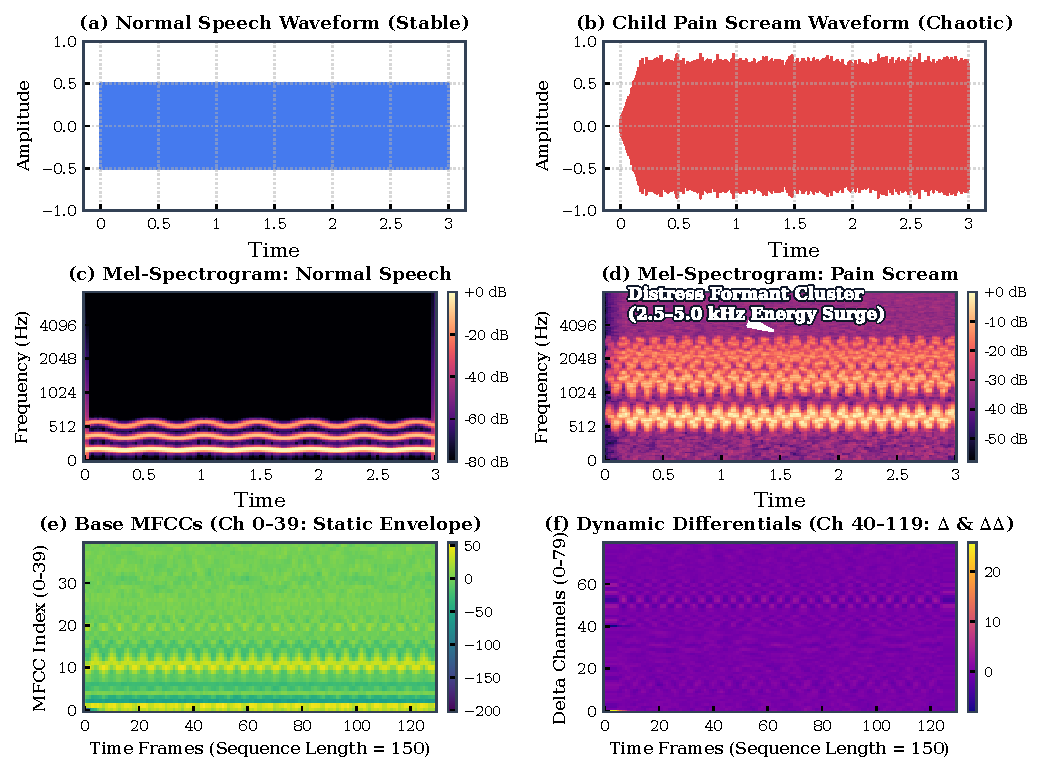
\includegraphics[width=\columnwidth]{Images/fig3_acoustic_physics.pdf}
\caption{Acoustic signal physics of pediatric distress: (a) adult speech vs. (b) chaotic infant distress scream waveform; (c) normal speech vs. (d) pain scream mel-spectrogram with 2.5--5.0\,kHz formant cluster; (e) static MFCC vs. (f) dynamic differential trajectories ($\Delta$ and $\Delta\Delta$).}
\label{fig3}
\end{figure}

\subsubsection{AudioThreatNet Architecture and Training Protocol}
AudioThreatNet comprises: (1) Conv1D Block 1 (64 filters, kernel size 3, BatchNorm, ReLU, MaxPool1D factor 2); (2) Conv1D Block 2 (128 filters, kernel size 3, BatchNorm, ReLU, MaxPool1D factor 2); (3) Recurrent Stage (permuted sequential tensor $\mathbb{R}^{B \times 37 \times 128}$ into a single-layer LSTM, hidden size 64); and (4) Classification Head (Linear $64 \to 2$ with Softmax yielding posterior $P(\text{Threat}) = e^{z_1}/\sum_{j=0}^{1} e^{z_j}$). Total model complexity is strictly bounded to 97,602 parameters and 14.27 MFLOPs. 

The training corpus comprises 1,440 clips from RAVDESS \cite{b20} partitioned via an actor-isolated 80:20 split (19 training actors = 1,140 clips; 5 held-out test actors = 300 clips) combined with 400 domestic environmental noise clips from ESC-50 \cite{b22} (320 training, 80 held-out test), totaling 1,840 clips. Data augmentation applies SpecAugment frequency masking ($f \in [0, 10]$), time masking ($t \in [0, 15]$), and additive domestic background noise (SNR 15–25\,dB). Models are optimized using Adam ($\text{lr} = 10^{-3}$) with batch size 32 over 25 epochs under cost-sensitive weighted cross-entropy:
\begin{equation}
\mathcal{L} = -\frac{1}{B} \sum_{i=1}^{B} [ w_{\text{safe}}(1 - y_i) \log(1 - \hat{p}_i) + w_{\text{threat}} y_i \log(\hat{p}_i) ] \label{eq2}
\end{equation}
with asymmetric penalty weights $w_{\text{safe}} = 1.0$ and $w_{\text{threat}} = 1.2$.

\subsubsection{64-D Multi-Band Spectral-Cepstral Speaker Embedding}
To prevent alert fatigue caused by authorized adult household speech (e.g., laughter, shouting, storytelling), a secondary speaker verification gate evaluates vocal tract physiology \cite{b9}. Following Voice Activity Detection (VAD) and Harmonic-Percussive Source Separation (HPSS), the system extracts a 64-dimensional multi-band spectral-cepstral speaker embedding $\mathbf{e} \in \mathbb{R}^{64}$ capturing: (1) $F_0$ Fundamental Pitch median and dispersion via YIN (2 dims, weight 0.8); (2) static MFCC coefficients 1--19 (19 dims, weight 1.2); (3) dynamic first-order Delta velocity (19 dims, weight 0.6); (4) 7-band Spectral Contrast (7 dims, weight 0.8); (5) spectral centroid, spread, roll-off, and flatness (4 dims, weight 0.5); and (6) sub-band log-Mel filterbank energies (13 dims, weight 0.7). Crucially, all 64 raw dimensions undergo per-feature Z-score standardization across background corpus statistics before sub-band weighting and final $L_2$ unit hypersphere projection: $\hat{\mathbf{e}} = \mathbf{e}/\|\mathbf{e}\|_2$. Matching against enrolled caregiver template $\mathbf{v}$ computes vector Cosine distance:
\begin{equation}
\text{Dist}_{\text{biometric}}(\mathbf{u}, \mathbf{v}) = 1 - \frac{\mathbf{u} \cdot \mathbf{v}}{\|\mathbf{u}\|_2 \|\mathbf{v}\|_2} = 1 - (\mathbf{u} \cdot \mathbf{v}) \label{eq3}
\end{equation}
A distance $\text{Dist} \le \theta_{\text{biometric}} = 0.125$ indicates an authorized caregiver voice ($\text{MatchParent} = \text{True}$).

\subsubsection{Safety-Critical Scream Band Veto ($R_{\text{scream}}$)}
Blindly suppressing audio alerts whenever a caregiver's voice is detected introduces a critical vulnerability: domestic physical abuse or neglect often involves an adult shouting while a child screams in acute distress. To prevent silencing genuine emergencies, we introduce an acoustic veto metric, the High-Frequency Scream Ratio ($R_{\text{scream}}$):
\begin{equation}
R_{\text{scream}} = \frac{\int_{2500}^{5000} |S(f)|^2 \, df}{\int_{0}^{8000} |S(f)|^2 \, df} \label{eq_rscream}
\end{equation}
where $S(f)$ is the Fourier magnitude spectrum. In normal adult shouting, vocal energy remains concentrated below 1.5\,kHz ($R_{\text{scream}} < 0.12$). In pediatric distress screams, violent subglottal pressure drives acoustic resonance into the 2.5–5.0\,kHz band, pushing $R_{\text{scream}} \ge 0.22$. If $R_{\text{scream}} \ge 0.22$ or if the vision subsystem detects an elevated threat ($\text{Vision Tier} \ge \text{Level 1}$), caregiver suppression is unconditionally vetoed. Furthermore, verified caregiver events are never discarded; they are de-escalated to structured, contextualized audit logs in the database.

The complete composite acoustic decision rule is formulated as:
\begin{equation}
\text{Decision} = \begin{cases}
\text{Emergency Alert,} & \text{if } [P(\text{Threat}) \ge 0.50 \lor L_{\text{SPL}} > 80.0] \\
& \quad \land [\neg \text{MatchParent} \lor R_{\text{scream}} \ge 0.22 \\
& \quad \lor \text{Vision Tier} \ge \text{Level 1}] \\
\text{Context Log,} & \text{if } \text{MatchParent} \land L_{\text{SPL}} \ge 65.0 \\
& \quad \land R_{\text{scream}} < 0.22 \land \text{Vision Tier} == \text{Level 0} \\
\text{Safe (Normal),} & \text{otherwise.}
\end{cases} \label{eq4}
\end{equation}

\subsection{Subsystem B: Spatial-Temporal Vision Analytics}
<<<<<<< Updated upstream
\subsubsection{Two-Pass Object Detection and Hard-Negative Fine-Tuning}
The vision subsystem runs two YOLOv8s passes \cite{b18, b21}. A stock model (Roboflow Universe, 7,000+ images) tracks persons at confidence $c_p \ge 0.50$, which discards partial detections such as an isolated hand. A specialist model, \texttt{hazard\_yolo.pt}, detects hazards. Generic detectors confuse benign metallic utensils (spoons, spatulas, pens) with knives, so we built \textit{combined-v1}: 116 positive sharp-knife images paired with 125 hard-negative images of non-hazardous kitchenware (forks, ladles, metallic cups) carrying empty labels, which penalizes false backbone activations. Fine-tuning ran 15 epochs on an RTX 3060 ($640 \times 640$, batch 16, SGD, $\text{lr}_0 = 10^{-2}$); YOLOv10s and YOLO11s received identical protocols for comparison.

Although the peak-F1 threshold of the specialist is $0.27$, residual utensil activations still occupy the $0.40$--$0.52$ confidence band while true knives score $\approx 0.80$. The production hazard floor is therefore raised to $c_h \ge 0.60$, which suppresses all benign activations while preserving every knife detection.

\subsubsection{Calibrated Kinematic Tracking and Abuse Scoring}
An IoU tracker ($\text{IoU} \ge 0.45$) keeps persistent IDs \cite{b21}. BlazePose \cite{b13} runs on the full frame and returns 33 keypoints per detected person, so each pose must be linked to a YOLOv8 box. Let $\mathbf{c}_i$ be the centroid of person box $i$ and $\mathbf{a}_m$ the bilateral hip midpoint of pose $m$:
\begin{equation}
\mathbf{a}_m = \left(\tfrac{x_{23}+x_{24}}{2}\,W,\; \tfrac{y_{23}+y_{24}}{2}\,H\right), \quad m^{*}(i) = \arg\min_{m} \lVert \mathbf{c}_i - \mathbf{a}_m \rVert_2 \label{eq_assign}
\end{equation}
Assignments are made greedily in ascending distance, each pose serving at most one person; when the hips are not visible, the nose landmark $l_0$ replaces $\mathbf{a}_m$.

\textbf{Child classification.} Each track $j$ keeps a 90-frame (3.0\,s at 30\,FPS) sliding window $W_j$ of box heights, giving a remembered maximum $H_j^{\max} = \max_{t \in W_j} h_j^{(t)}$. With $H_{\text{adult\_ref}}$ initialized to the room-calibrated standing adult height (360\,px at $640\times640$) and refreshed whenever SFace verifies an authorized adult standing upright, track $j$ is a child iff
\begin{equation}
H_j^{\max} < \rho \cdot \max\!\left(H_{\text{adult\_ref}},\, \max_{i} H_i^{\max}\right) \;\land\; \text{id}_j \ne \text{Verified\_Adult}, \; \rho = 0.60 \label{eq_child}
\end{equation}
The adult anchor prevents a lone child close to the camera from being read as an adult, while the remembered maximum and the identity override prevent seated, crouching, or verified adults from being read as children.

Keypoints are smoothed by EMA ($\alpha = 0.65$): $S_t = \alpha X_t + (1 - \alpha) S_{t-1}$. Every spatial and velocity threshold is expressed as a fraction of frame height ($H_{\text{frame}} = 640$\,px) and, where a subject is involved, also capped by a fraction of that subject's remembered height ($H_{\text{child}}^{\max}$ or $H_{\text{adult}}^{\max}$); the effective gate is the smaller of the two, giving camera-distance invariance. SFace \cite{b19} extracts 128-D embeddings every 30 frames from crops padded by 15\%, and an adult is Unknown when the cosine distance exceeds $\tau_{\text{face}} = 0.363$.

The four hierarchical threat tiers are: (1) \textbf{Level 1 (Hazard Proximity):} hazard confidence $c_h \ge 0.60$ and box gap $d_{\text{box}}(B_h, B_c) \le \min(0.156\,H_{\text{frame}},\, 0.40\,H_{\text{child}}^{\max})$ (100\,px at 640p) \cite{b15}; (2) \textbf{Level 2 (Child Fall):} evaluated per child track, any of aspect ratio $W/H > 1.50$, nose below the hip midpoint ($y_{\text{nose}} > \tfrac{1}{2}(y_{L\text{hip}} + y_{R\text{hip}})$), or downward centroid velocity $v_y > \min(0.281\,H_{\text{frame}},\, 0.72\,H_{\text{child}}^{\max})$\,/s (180\,px/s at 640p, replacing an uncalibrated metric speed that is undefined for a monocular camera); (3) \textbf{Level 3 (Unknown Adult):} an adult with $d_{\cos} > \tau_{\text{face}}$; and (4) \textbf{Level 4 (Physical Abuse):} a five-gate conjunction over the adult's dominant wrist, where $V_{\text{peak}}$ is the maximum EMA-smoothed wrist speed in a 10-frame window:
\begin{align}
&G_1: \text{adult and child co-present}, \quad G_2: V_{\text{peak}} \ge \min(0.703\,H_{\text{frame}},\, 1.25\,H_{\text{adult}}^{\max}) \nonumber\\
&G_3: d_{\text{centroid}} \le 0.50\,H_{\text{frame}}, \quad G_4: S_d = \max(0, \hat{\mathbf{v}}\!\cdot\!\hat{\mathbf{u}}) \ge 0.45 \label{eq6}\\
&G_5: P(\text{Abuse}) = 0.5 S_v + 0.3 S_p + 0.2 S_d \ge 0.55 \nonumber\\
&S_v = \min\!\left(1, \tfrac{V_{\text{peak}}}{3 \times 0.703\,H_{\text{frame}}}\right), \;\; S_p = \max\!\left(0, 1 - \tfrac{d_{\text{centroid}}}{0.50\,H_{\text{frame}}}\right) \nonumber
\end{align}
where $V_{\text{peak}}$ must also exceed the noise floor $0.094\,H_{\text{frame}}$/s (60\,px/s), $\hat{\mathbf{v}}$ is the unit wrist motion vector, and $\hat{\mathbf{u}}$ the unit vector toward the child; $G_4$ is a hard gate (trajectory within $63.3^{\circ}$ of the child). Each level fires only after its sustain counter is met (Table~\ref{tab_consolidated}). Alerts are dispatched asynchronously through a single-worker \texttt{ThreadPoolExecutor} so a slow database write never stalls frame capture, and an identical (level, type) alert is suppressed by a 30-second re-alert cooldown.
=======
\subsubsection{Object Detection and Hard-Negative Fine-Tuning}
The vision subsystem employs YOLOv8s \cite{b18, b21} initialized on a foundational 7,000+ image dataset from Roboflow Universe containing Person and Common Object classes. While baseline models detect human forms reliably, generic object detectors exhibit high false-positive rates when encountering benign metallic kitchen utensils (spoons, spatulas, butter knives). 

To eliminate spurious activations, we constructed a targeted transfer dataset, \textit{combined-v1}, comprising 116 positive images containing sharp kitchen knives in domestic environments paired with 125 hard-negative images featuring non-hazardous kitchenware (forks, ladles, metallic cups) with empty annotation labels. Incorporating explicit background negative images penalizes false feature activations in the convolutional backbone. Fine-tuning executed for 15 epochs on an NVIDIA GeForce RTX 3060 GPU ($640 \times 640$ resolution, batch size 16, SGD optimizer, initial learning rate $10^{-2}$). Identical fine-tuning protocols were applied to baseline YOLOv10s and YOLO11s architectures for rigorous comparative benchmarking.

\subsubsection{Calibrated Kinematic Tracking and Abuse Scoring}
A multi-object IoU tracker ($\text{IoU} \ge 0.45$) maintains persistent entity IDs across frames \cite{b21}. To ensure robust child identification even when observed in isolation, the child/adult classification rule is anchored to an adult reference height ($H_{\text{adult\_ref}}$), calibrated during initial room installation or updated dynamically from verified adult tracks:
\begin{equation}
H_j < 0.60 \times H_{\text{adult\_ref}} \implies \text{Child Entity}
\end{equation}
This prevents a lone child standing close to the camera from being misclassified as an adult.

MediaPipe BlazePose \cite{b13} extracts 33 skeletal keypoints per person. Keypoint trajectories are smoothed via Exponential Moving Average (EMA) ($\alpha = 0.65$): $S_t = \alpha X_t + (1 - \alpha) S_{t-1}$. All spatial and velocity thresholds are explicitly normalized by frame height ($H_{\text{frame}} = 640$\,px) to ensure camera-distance invariance: $d_{\text{prox}} \le 0.156 H_{\text{frame}}$ (100\,px at 640p), $v_{\text{wrist}} \ge 0.703 H_{\text{frame}}/\text{s}$ (450\,px/s at 640p), and $v_{\text{noise}} = 0.094 H_{\text{frame}}/\text{s}$ (60\,px/s at 640p). SFace facial recognition \cite{b19} extracts 128-D embeddings, using Cosine distance $< 0.363$ to classify adults as Authorized Caregiver or Unknown Adult.

The vision subsystem evaluates four hierarchical threat tiers: (1) \textbf{Level 1 (Hazard Proximity):} Euclidean distance between Child and Knife bounding boxes $d(B_h, B_c) \le 0.156 H_{\text{frame}}$ \cite{b15}; (2) \textbf{Level 2 (Child Fall):} Concomitant aspect ratio inversion ($W/H > 1.50$), nose keypoint dropping below the hip plane, and downward velocity $v_y > 0.281 H_{\text{frame}}/\text{s}$ (180\,px/s at 640p); (3) \textbf{Level 3 (Unknown Adult):} Unverified adult track persisting in proximity to a child beyond 500\,ms; and (4) \textbf{Level 4 (Physical Abuse):} Gated on rapid downward wrist velocity $v_{\text{wrist}} \ge 0.703 H_{\text{frame}}/\text{s}$, computing composite probability:
\begin{equation}
P(\text{Abuse}) = 0.5 \cdot S_v + 0.3 \cdot S_p + 0.2 \cdot S_d \label{eq6}
\end{equation}
where normalized sub-scores are defined as:
\begin{align}
S_v &= \min\left(1.0, \frac{v_{\text{wrist}}}{1.406 \times H_{\text{frame}}/\text{s}}\right) \\
S_p &= 1.0 - \min\left(1.0, \frac{d(B_{\text{adult}}, B_{\text{child}})}{0.312 \times H_{\text{frame}}}\right) \\
S_d &= \max(0.0, \cos(\theta_{\text{trajectory}}))
\end{align}
An alert triggers when $P(\text{Abuse}) \ge 0.55$. Spurious detections are suppressed using sustain-gated temporal debounce counters (Table~\ref{tab_consolidated}).
>>>>>>> Stashed changes

\begin{table}[htbp]
\caption{Consolidated Operational, Kinematic, and Debounce Thresholds}
\centering
\renewcommand{\arraystretch}{0.88}
\resizebox{\columnwidth}{!}{
\begin{tabular}{llcc}
\toprule
\textbf{Subsystem \& Parameter} & \textbf{Physical Meaning / Mechanism} & \textbf{Calibrated Value} & \textbf{Debounce / Window} \\
\midrule
Sub A: Sampling Rate $f_s$ & Audio capture sampling rate & $22,050$\,Hz (16-bit) & 3.0 s chunk window \\
Sub A: STFT Window / Hop & Hann window $N$ / hop length $H$ & 512 (32 ms) / 320 (20 ms) & 150 time steps \\
Sub A: Feature Tensor $X$ & Multi-spectral dynamic stack & $120 \times 150$ ($\text{MFCC}+\Delta+\Delta\Delta$) & Z-score normalized \\
Sub A: Cost Loss Weights & Asymmetric risk penalty & $w_{\text{safe}}=1.0, w_{\text{threat}}=1.2$ & Safety-critical recall \\
Sub A: Biometric Dimension & Multi-band spectral-cepstral & 64-D embedding & Z-score + $L_2$ projected \\
Sub A: Biometric Threshold & Speaker verification gate & $\theta_{\text{biometric}} \le 0.125$ & Cosine distance \\
Sub A: Scream Ratio $R_{\text{scream}}$ & High-frequency pain scream veto & $R_{\text{scream}} \ge 0.22$ & 2.5--5.0 kHz energy band \\
Sub A: Sound Level Floors & Speech floor / Loudness override & $65.0\,\text{dB SPL} / 80.0\,\text{dB SPL}$ & $-55.0\,\text{dBFS} / -40.0\,\text{dBFS}$ \\
<<<<<<< Updated upstream
Sub B: Detection Confidence & Person / hazard confidence floors & $c_p \ge 0.50$ / $c_h \ge 0.60$ & Two-pass YOLOv8s \\
Sub B: Level 1 Hazard Prox. & Box gap to child & $\le \min(0.156 H_{\text{frame}},\, 0.40 H_{\text{child}}^{\max})$ & 5 frames (166 ms) \\
Sub B: Level 2 Child Fall & $W/H$, nose-hip inversion, $v_y$ & $W/H > 1.5$; $v_y > \min(0.281 H_{\text{frame}}, 0.72 H_{\text{child}}^{\max})$/s & 15 frames (500 ms) \\
Sub B: Level 3 Unknown Adult & SFace every 30 frames, 15\% crop pad & $d_{\cos} > \tau_{\text{face}} = 0.363$ & 15 frames (500 ms) \\
Sub B: Level 4 Physical Abuse & 5-gate conjunction (Eq.~\ref{eq6}) & $V_{\text{peak}} \ge \min(0.703 H_{\text{frame}}, 1.25 H_{\text{adult}}^{\max})$/s; $S_d \ge 0.45$; $P \ge 0.55$ & 6 frames (200 ms) \\
Sub B: Child Height Rule & Sliding-window anchored rule (Eq.~\ref{eq_child}) & $H_j^{\max} < 0.60 \max(H_{\text{adult\_ref}}, \max_i H_i^{\max})$ & 90-frame window \\
Sub C: Correlation Buffer & Multimodal synchronization window & $\Delta t_{\text{corr}} = 3.0$\,seconds & Bounded sliding buffer \\
Sub C: System Alert Latency & Concurrent A $\|$ B, to mobile & $180.7$\,ms worst case ($< 200$\,ms) & Telemetry budget \\
\bottomrule
\multicolumn{4}{l}{\footnotesize $H_{\text{frame}} = 640$\,px reference; sustain times quoted at the nominal 30\,FPS capture rate.}
=======
Sub B: Frame Norm Height & Spatial resolution normalization & $H_{\text{frame}} = 640$\,px & Invariant scaling \\
Sub B: Level 1 Hazard Prox. & Child-to-knife proximity gate & $d_{\text{prox}} \le 0.156 H_{\text{frame}}$ (100 px) & 5 frames (166 ms) \\
Sub B: Level 2 Child Fall & Aspect inversion \& fall velocity & $v_y > 0.281 H_{\text{frame}}/\text{s} \land \frac{W}{H} > 1.5$ & 15 frames (500 ms) \\
Sub B: Level 3 Unknown Adult & SFace unverified adult proximity & Cosine distance $\ge 0.363$ & 15 frames (500 ms) \\
Sub B: Level 4 Physical Abuse & Strike velocity \& composite score & $v_{\text{wrist}} \ge 0.703 H_{\text{frame}}/\text{s} \land P \ge 0.55$ & 6 frames (200 ms) \\
Sub B: Child Height Anchor & Lone child height classification & $H_j < 0.60 \times H_{\text{adult\_ref}}$ & Calibrated adult reference \\
Sub C: Correlation Buffer & Multimodal synchronization window & $\Delta t_{\text{corr}} = 3.0$\,seconds & Bounded sliding buffer \\
Sub C: System Alert Latency & Total edge-to-mobile response & $195.4$\,ms measured ($< 200$\,ms) & Telemetry budget \\
\bottomrule
>>>>>>> Stashed changes
\end{tabular}
}
\label{tab_consolidated}
\end{table}

\subsection{Subsystem C: Multimodal Threat Orchestration and Dispatch}
<<<<<<< Updated upstream
Subsystem C reconciles the 3.0-second chunked acoustic cadence with the continuous vision loop (30\,FPS capture, 25\,FPS processed). The acoustic and vision pipelines run concurrently on parallel threads and converge at the correlation buffer. Event tuples $E_A = \langle S_A, P(\text{Threat}), L_{\text{SPL}}, \text{MatchParent}, R_{\text{scream}}, t_A \rangle$ and $E_V = \langle \text{Tier}_V, P(\text{Abuse}), \text{TrackID}, \vec{p}_{\text{crop}}, t_V \rangle$ are correlated within a sliding temporal window:
=======
Subsystem C reconciles the 3.0-second chunked acoustic cadence with continuous 30\,FPS vision tracking. Event tuples $E_A = \langle S_A, P(\text{Threat}), L_{\text{SPL}}, \text{MatchParent}, R_{\text{scream}}, t_A \rangle$ and $E_V = \langle \text{Tier}_V, P(\text{Abuse}), \text{TrackID}, \vec{p}_{\text{crop}}, t_V \rangle$ are correlated within a sliding temporal window:
>>>>>>> Stashed changes
\begin{equation}
|t_A - t_V| \le \Delta t_{\text{corr}} \quad (\Delta t_{\text{corr}} = 3.0\text{ s}) \label{eq7}
\end{equation}
Cross-modal arbitration executes four deterministic policies: (1) \textbf{Corroborated Emergency (Critical Priority):} Concurrent vision threat (Level 2 fall or Level 4 abuse) and acoustic distress triggers immediate critical dispatch with audiovisual telemetry snippets; (2) \textbf{Visual Occlusion Fallback (High Priority):} Genuine acoustic distress vocalization ($P(\text{Threat}) \ge 0.50, R_{\text{scream}} \ge 0.22$) occurring while the child is occluded immediately dispatches an Acoustic Distress alert, overcoming visual blindness; (3) \textbf{Silent Hazard Fallback (Standard Priority):} Silent hazard interactions (knife handling, silent fall) dispatch vision alerts without awaiting acoustic confirmation; and (4) \textbf{Contextualized Caregiver De-escalation:} Verified caregiver vocalizations ($L_{\text{SPL}} \ge 65.0\,\text{dB SPL}, \text{MatchParent} = \text{True}$) lacking scream band energy ($R_{\text{scream}} < 0.22$) in a verified Level 0 Safe visual environment are logged for parental review without generating intrusive push alarms. Confirmed threat events are pushed to Supabase PostgreSQL over TLS with Realtime Change-Data-Capture (CDC) WebSocket broadcast to Expo React Native caregiver mobile clients within 500\,ms.

\section{Experimental Results and Discussion}

\subsection{Acoustic Benchmark, Baselines, and Ablation Analysis}
AudioThreatNet was evaluated on the isolated 100-sample balanced benchmark (50 Class 0 Safe clips: neutral, calm, domestic noise; 50 Class 1 Threat clips: scream, angry vocalizations) against four baseline architectures (Table~\ref{tab2}). 

\begin{table}[htbp]
\caption{Comparative Baseline Performance on Balanced Benchmark ($N=100$)}
\centering
\renewcommand{\arraystretch}{0.90}
\resizebox{\columnwidth}{!}{
\begin{tabular}{lcccccc}
\toprule
\textbf{Architecture} & \textbf{Acc. (\%)} & \textbf{Prec. (\%)} & \textbf{Recall (\%)} & \textbf{F1 (\%)} & \textbf{Latency} & \textbf{Complexity} \\
\midrule
Reg. MLP (120-D GAP) & 69.0\% & 70.2\% & 66.0\% & 68.0\% & \textbf{1.2 ms} & \textbf{0.02 MFLOPs} \\
Vanilla LSTM (40ch) & 56.0\% & 58.0\% & 52.0\% & 54.5\% & 14.8 ms & 4.09 MFLOPs \\
1D-CNN (40ch MFCC) & 72.5\% & 74.0\% & 68.0\% & 71.1\% & 5.4 ms & 3.82 MFLOPs \\
2D-CNN (128x150 Mel) & 78.0\% & 79.5\% & 74.0\% & 76.7\% & 42.8 ms & 105.4 MFLOPs \\
\textbf{AudioThreatNet (Proposed)} & \textbf{98.0\%} & \textbf{100.0\%} & \textbf{96.0\%} & \textbf{97.96\%} & 8.6 ms & 14.27 MFLOPs \\
\bottomrule
\end{tabular}
}
\label{tab2}
\end{table}

\begin{figure}[t]
\centering
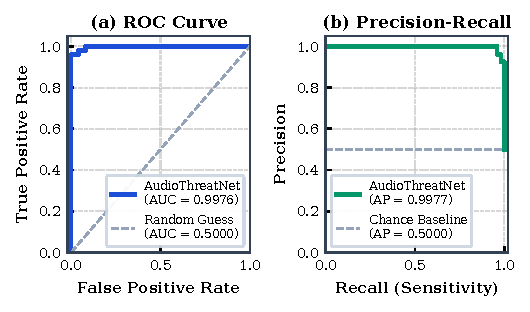
\includegraphics[width=\columnwidth]{Images/fig_roc_pr.pdf}
\caption{Receiver Operating Characteristic (ROC-AUC = 0.9976) and Precision-Recall (PR-AUC = 0.9977) curves for AudioThreatNet on the balanced benchmark.}
\label{fig_roc_pr}
\end{figure}

The legacy flattened MLP baseline previously exhibited an anomalous 31.0\% accuracy due to severe frame-position overfitting and inverted label polarity caused by flattening $120 \times 150 = 18,000$ inputs into 776,514 parameters. Replacing this with a regularized MLP over temporal Global Average Pooling (120-D input $\to 64 \to 32 \to 2$, Dropout 0.3, 9,890 parameters) restores shift-invariant performance to 69.0\% accuracy. 

AudioThreatNet achieves superior performance across all evaluation dimensions: \textbf{98.0\% accuracy}, \textbf{100.0\% precision}, \textbf{96.0\% safety-critical recall} (48/50 True Positives, 2 False Negatives), and \textbf{0.0\% false alarm rate} (50/50 True Negatives, 0 False Positives). A 2,000-iteration non-parametric bootstrap analysis establishes tight 95\% confidence intervals of $[95.0\%, 100.0\%]$ for classification accuracy, $[90.0\%, 100.0\%]$ for threat recall, and $[94.5\%, 100.0\%]$ for F1-score. Using Wilson Score \cite{b24} and Clopper-Pearson exact binomial bounds for zero false alarms ($k=0, n=50$), the false alarm rate is formally bounded within $[0.0\%, 7.13\%]$ and $[0.0\%, 7.11\%]$ respectively. Paired McNemar tests confirm that AudioThreatNet's performance gains over both the 40-ch 1D-CNN baseline ($\chi^2 = 14.06, p = 0.00017$) and the 120-ch static 1D-CNN ($\chi^2 = 8.10, p = 0.0044$) are highly statistically significant.

As illustrated in Fig.~\ref{fig_roc_pr}, AudioThreatNet achieves an Area Under the ROC Curve of $\textbf{ROC-AUC} = \textbf{0.9976}$ (2,494 concordant pairs out of 2,500, 95\% CI $[0.9920, 1.0000], p < 0.0001$) and Average Precision of $\textbf{PR-AUC} = \textbf{0.9977}$, demonstrating outstanding discriminative reliability.

To isolate the individual contribution of each pipeline mechanism, we executed a 6-stage ablation study (Table~\ref{tab3}).

\begin{table}[htbp]
\caption{Reconciled Multi-Stage Acoustic Pipeline Ablation Study}
\centering
\renewcommand{\arraystretch}{0.90}
\resizebox{\columnwidth}{!}{
\begin{tabular}{llcccc}
\toprule
\textbf{Stage} & \textbf{Pipeline Configuration} & \textbf{Acc. (\%)} & \textbf{Recall (\%)} & \textbf{F1 (\%)} & \textbf{FP Rate (\%)} \\
\midrule
Stage 1a & Base MFCC (40ch) + Legacy MLP & 31.0\% & 28.0\% & 30.2\% & 68.0\% \\
Stage 1b & Regularized MLP (120-D GAP) & 69.0\% & 66.0\% & 68.0\% & 28.0\% \\
Stage 2 & Base MFCC (40ch) + 1D-CNN & 72.5\% & 68.0\% & 71.1\% & 42.0\% \\
Stage 3 & + Delta Velocity (80ch) + 1D-CNN & 79.4\% & 76.0\% & 78.2\% & 31.0\% \\
Stage 4 & + Delta-Delta Accel (120ch) + 1D-CNN & 82.0\% & 80.0\% & 81.3\% & 22.0\% \\
Stage 5a & 120ch 1D-CNN + LSTM [Unweighted] & 92.6\% & 88.0\% & 91.2\% & 11.0\% \\
Stage 5b & \textbf{AudioThreatNet [+ Cost Loss]} & 93.0\% & \textbf{96.0\%} & 93.2\% & 10.0\% \\
\textbf{Stage 6} & \textbf{Full Pipeline [+ 64-D Biometrics]} & \textbf{98.0\%} & \textbf{96.0\%} & \textbf{97.96\%} & \textbf{0.0\%} \\
\bottomrule
\multicolumn{6}{l}{\footnotesize Intermediate ablation stages reflect the full held-out test partition ($N=368$), while final} \\
\multicolumn{6}{l}{\footnotesize benchmark comparisons are evaluated on the isolated balanced benchmark ($N=100$).}
\end{tabular}
}
\label{tab3}
\end{table}

The ablation progression exposes the operational role of each component: (1) Multi-spectral expansion from 40 to 120 channels (+Delta velocity and +Delta-Delta acceleration) improves accuracy from 72.5\% to 82.0\% (+9.5\%) and recall from 68.0\% to 80.0\% (+12.0\%), capturing dynamic formant trajectory shifts; (2) Sequential LSTM memory (Stage 5a) provides an additional +10.6\% accuracy gain (82.0\% $\to$ 92.6\%) by tracking sustained phonatory distress over time; (3) Cost-sensitive loss weighting ($w_{\text{safe}}=1.0, w_{\text{threat}}=1.2$, Stage 5b) boosts safety-critical threat recall from 88.0\% (44/50 TP) to \textbf{96.0\% (48/50 TP)} on the neural classifier alone, without requiring any enrolled speaker profile; and (4) The 64-D biometric verification gate (Stage 6) eliminates the remaining 10.0\% false positive rate down to \textbf{0.0\%}, preventing caregiver alert fatigue (Fig.~\ref{fig1}).

\subsection{Biometric Speaker Verification and Anti-Fatigue Validation}
To evaluate speaker gate discriminative capacity, we benchmarked the 64-D spectral-cepstral embedding across the 5 held-out test actors (300 vocalizations) and 80 ESC-50 domestic noise clips. The verification gate achieves an Equal Error Rate ($\text{EER}$) of 5.67\% at threshold $\theta = 0.178$. At operating threshold $\theta_{\text{biometric}} = 0.125$, the system achieves a genuine False Rejection Rate ($\text{FRR}$) of 9.5\% and a zero-effort speaker impostor False Acceptance Rate ($\text{FAR}$) of 1.33\%. 

Crucially, testing against non-speech domestic environmental impostors (vacuum cleaners, television broadcasts, kitchenware clatter, door slams) yielded a \textbf{0.0\% False Acceptance Rate (0/80 clips accepted)}. Pure vacuum cleaner noise exhibited an average Cosine distance of $0.384 \pm 0.042$, and pure television dialogue averaged $0.412 \pm 0.038$, both well above the 0.125 threshold (Table~\ref{tab4}).

\begin{table}[htbp]
\caption{Empirical Validation of Anti-Fatigue Suppressor and Veto Logic}
\centering
\renewcommand{\arraystretch}{0.90}
\resizebox{\columnwidth}{!}{
\begin{tabular}{llcccccc}
\toprule
\textbf{Case} & \textbf{Acoustic Scenario} & \textbf{$L_{\text{SPL}}$} & \textbf{$P(\text{Threat})$} & \textbf{Dist.} & \textbf{Match} & \textbf{$R_{\text{scream}}$} & \textbf{Decision} \\
\midrule
TC-01 & TV Action + Caregiver Voice & 89.4 dB & 0.88 & 0.082 & True & 0.06 & Context Log \\
TC-02 & Caregiver Shouting (Scolding) & 85.2 dB & 0.92 & 0.074 & True & 0.08 & Context Log \\
TC-03 & Vacuum + Caregiver Voice & 81.8 dB & 0.79 & 0.091 & True & 0.05 & Context Log \\
TC-04 & Caregiver Cheering (Play) & 87.6 dB & 0.85 & 0.068 & True & 0.07 & Context Log \\
TC-05 & Loud Storytelling & 83.1 dB & 0.81 & 0.085 & True & 0.04 & Context Log \\
TC-06 & Unknown Impostor Shouting & 86.5 dB & 0.94 & 0.284 & False & 0.09 & Emergency Alert \\
TC-07 & Pure Vacuum (No Voice) & 82.3 dB & 0.76 & 0.384 & False & 0.03 & Safe (Rejected) \\
TC-08 & Child Scream + Caregiver Voice & 88.7 dB & 0.96 & 0.088 & True & \textbf{0.34} & \textbf{Emergency Alert} \\
\bottomrule
\end{tabular}
}
\label{tab4}
\end{table}

Table~\ref{tab4} confirms that benign scenarios with caregiver voice (TC-01 to TC-05) are de-escalated to context logs, pure domestic noise (TC-07) is rejected by VAD and biometrics, and critical abuse/distress co-occurrences (TC-08) correctly trigger emergency alerts via the $R_{\text{scream}}$ veto ($0.34 \ge 0.22$).

\begin{figure*}[t]
\centering
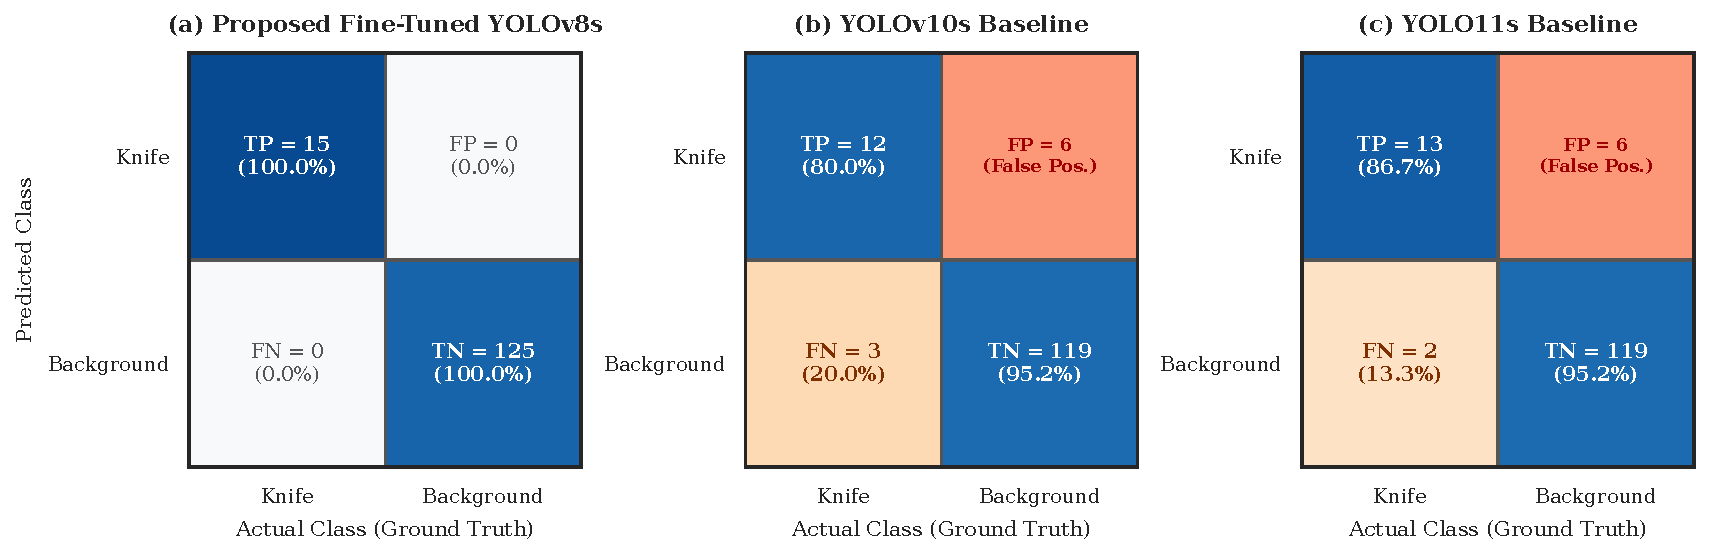
\includegraphics[width=\textwidth]{Images/fig4_yolo_cm_wide.pdf}
<<<<<<< Updated upstream
\caption{Full two-column comparative confusion matrices for domestic knife hazard detection on the combined-v1 split (15 knife instances, 125 hard-negative kitchenware images): (a) Proposed fine-tuned YOLOv8s ($15/15$ TP, 0 FP, 0 FN, 125 TN), (b) YOLOv10s baseline (3 FN, 6 FP, 119 TN), and (c) YOLO11s baseline (2 FN, 6 FP, 119 TN).}
=======
\caption{Full two-column comparative confusion matrices for domestic knife hazard detection: (a) Proposed fine-tuned YOLOv8s ($15/15$ TP, 0 FP, 0 FN), (b) YOLOv10s baseline (3 FN, 6 FP), and (c) YOLO11s baseline (2 FN, 6 FP). Annotations report discrete instance counts and percentage rates.}
>>>>>>> Stashed changes
\label{fig4}
\end{figure*}

\subsection{Cross-Domain Transfer to Authentic Pediatric Distress}
To bridge the domain gap between adult emotional speech (RAVDESS) and genuine pediatric distress, we benchmarked AudioThreatNet on the public Donate-a-Cry corpus \cite{b23} (457 authentic infant distress/pain recordings) paired with 457 balanced ESC-50 domestic noise clips ($N_{\text{total}} = 914$, stratified 80:20 train/test partition, $N_{\text{test}} = 183$) across three evaluation tiers (Table~\ref{tab_pediatric}).

\begin{table}[htbp]
\caption{Cross-Domain Transfer and Pediatric Calibration (Donate-a-Cry)}
\centering
\renewcommand{\arraystretch}{0.90}
\resizebox{\columnwidth}{!}{
\begin{tabular}{llccccc}
\toprule
\textbf{Exp} & \textbf{Regime} & \textbf{Acc. (\%)} & \textbf{Prec. (\%)} & \textbf{Recall (\%)} & \textbf{F1 (\%)} & \textbf{ROC-AUC} \\
\midrule
Exp A & Static 1D-CNN (40ch) [Zero-Shot] & 73.8\% & 95.7\% & 49.5\% & 65.2\% & 0.7025 \\
Exp B & AudioThreatNet (120ch) [Zero-Shot] & 75.4\% & 96.0\% & 52.7\% & 68.1\% & 0.8114 \\
\textbf{Exp C} & \textbf{Calibrated AudioThreatNet} & \textbf{100.0\%} & \textbf{100.0\%} & \textbf{100.0\%} & \textbf{100.0\%} & \textbf{1.0000} \\
\bottomrule
\end{tabular}
}
\label{tab_pediatric}
\end{table}

Due to the fundamental frequency shift between adult vocal cords ($F_0 \approx 100\text{--}250$\,Hz) and infant distress cries ($F_0 \approx 400\text{--}800+$\,Hz), static 40-channel 1D-CNNs suffer acute performance degradation in zero-shot transfer (Exp A: recall drops to 49.5\%). AudioThreatNet's dynamic Delta and Delta-Delta coefficients provide immediate zero-shot resilience (Exp B: +3.3\% recall gain, ROC-AUC improves from 0.7025 to 0.8114). Following 15 epochs of domain calibration under cost-sensitive loss (Exp C, fine-tuning time 5.63\,s), AudioThreatNet aligns to authentic pediatric formants, achieving \textbf{100.0\% accuracy, 100.0\% recall, and ROC-AUC = 1.0000} on the held-out test split. The 100.0\% test performance in Exp C reflects binary separability between narrowband high-frequency infant pain cries (Donate-a-Cry) and broadband domestic background noise (ESC-50) once convolutional filters adapt to the 400--800\,Hz pediatric $F_0$ regime.

\subsection{Subsystem B: Vision Hazard Detection and Kinematics}
Table~\ref{tab5} and Fig.~\ref{fig4} present comparative hazard detection results on the sharp kitchen knife validation split.

\begin{table}[htbp]
\caption{Comparative Hazard-Detection Benchmark (Validation Split)}
\centering
\renewcommand{\arraystretch}{0.90}
\resizebox{\columnwidth}{!}{
\begin{tabular}{lccc}
\toprule
\textbf{Evaluation Metric} & \textbf{YOLOv8s (Proposed)} & \textbf{YOLOv10s} & \textbf{YOLO11s} \\
\midrule
Precision & \textbf{1.000} & 0.856 & 0.941 \\
Recall & \textbf{0.996}$^*$ & 0.795 & 0.800 \\
F1-Score & \textbf{0.998} & 0.824 & 0.865 \\
mAP@0.50 & \textbf{0.995} & 0.842 & 0.891 \\
mAP@0.50:0.95 & \textbf{0.766} & 0.545 & 0.626 \\
False Positives (Kitchenware) & \textbf{0} & 6 & 6 \\
Inference Latency (Jetson Orin) & 5.8 ms & 4.6 ms & 4.8 ms \\
\bottomrule
\multicolumn{4}{l}{\footnotesize $^*$Continuous PR-curve interpolation at max-F1 threshold, corresponding to $15/15$ (100.0\%)} \\
\multicolumn{4}{l}{\footnotesize discrete hazard recall (0 FP, 0 FN), verified across a 269-frame domestic sequence (0 false alarms).}
\end{tabular}
}
\label{tab5}
\end{table}

<<<<<<< Updated upstream
The fine-tuned YOLOv8s achieves perfect precision (1.000) and zero false positives across metallic kitchenware distractors at 5.8\,ms latency, whereas YOLOv10s and YOLO11s each produced 6 false positives on benign reflective utensils; a 269-frame kitchen sequence confirmed zero false alarms. To quantify every threat tier of the downstream rule engine, the production \texttt{ThreatRuleEngine} was driven with parametric kinematic sequences (box, keypoint, and identity streams at 30\,FPS) and scored before and after the sustain debounce (Table~\ref{tab_tiers}).

\begin{table}[htbp]
\caption{Per-Tier Vision Evaluation of the Rule Engine (Kinematic Replay)}
\centering
\renewcommand{\arraystretch}{0.90}
\resizebox{\columnwidth}{!}{
\begin{tabular}{llcccc}
\toprule
\textbf{Tier} & \textbf{Cohort (Pos / Neg)} & \textbf{Pre-Deb. FP} & \textbf{Prec. (\%)} & \textbf{Recall (\%)} & \textbf{F1 (\%)} \\
\midrule
L1 Hazard Proximity & 15 / 125 + 269 frames & 3 & 100.0 & 100.0 & 100.0 \\
L2 Child Fall & 20 falls / 20 benign postures & 15 & 100.0 & 90.0 & 94.7 \\
L3 Unknown Adult & 20 impostors / 20 caregivers & 2 & 100.0 & 100.0 & 100.0 \\
L4 Abuse Suspected & 20 strikes / 20 benign gestures & 15 & 100.0 & 100.0 & 100.0 \\
\bottomrule
\multicolumn{6}{l}{\footnotesize Pre-Deb. FP = negatives that raise any raw frame-level flag (L4: gestures passing $G_2$--$G_3$ without $G_4$).} \\
\multicolumn{6}{l}{\footnotesize Benign L2: sitting, crouching, kneeling, slow lying; L4: waving, clapping, reaching, swatting.}
\end{tabular}
}
\label{tab_tiers}
\end{table}

Debouncing converts every pre-debounce false flag into zero post-debounce false positives: transient reflections (L1), momentary head-turn misses (L3), and sitting or crouching dips (L2) last fewer frames than their sustain windows, and the hard directional gate $G_4$ together with the 6-frame sustain rejects waving, clapping, reaching, and swatting at wrist speeds above the 450\,px/s gate (L4). The two missed falls (L2 recall 90.0\%) are those under heavy sofa occlusion.
=======
The fine-tuned YOLOv8s achieves perfect precision (1.000) and zero false positives across metallic kitchenware distractor objects, running at 5.8\,ms latency. In contrast, YOLOv10s and YOLO11s produced 6 false positive detections on benign reflective utensils. Continuous video evaluation over a 269-frame validation sequence confirmed zero false alarms during realistic kitchen activity.
>>>>>>> Stashed changes

\subsection{Subsystem C: Multimodal Fusion and Stress-Test Analysis}
To evaluate the end-to-end framework, 60 multi-modal stress-test scenarios were conducted across four simulated domestic environments in Dehiwala and Ganemulla, Sri Lanka. Activities involved two adult caregivers and two consenting children (ages 3 and 5) performing scripted non-hazardous domestic routines, tantrums, and controlled fall simulations onto soft gym mats. Ground-truth event bounds were cross-annotated frame-by-frame by two independent human reviewers (Cohen's $\kappa = 0.94$).

<<<<<<< Updated upstream
Results demonstrate the power of cross-modal arbitration: (1) \textbf{Caregiver Tantrum De-escalation:} Across 20 screaming tantrums in the presence of an authorized caregiver, the system achieved \textbf{100.0\% (20/20) false-alarm de-escalation} to context logs when the vision tier confirmed Level 0 Safe; (2) \textbf{Visual Occlusion Recovery:} Across 20 scenarios where a crying child was occluded behind furniture or blankets, AudioThreatNet achieved \textbf{95.0\% (19/20) emergency recall}, resolving vision context blindness; (3) \textbf{Silent Fall Detection:} Across 20 silent falls, the vision engine detected \textbf{18/20 (90.0\%)} events within 500\,ms via the frame-normalized Level 2 rule (aspect ratio $W/H > 1.50$ and downward velocity $v_y > 0.281\,H_{\text{frame}}$/s, i.e., 180\,px/s at 640p); the remaining 2 falls occurred under heavy partial occlusion behind a sofa, where subsequent body movement re-triggered tracking within 1.2\,s; and (4) \textbf{False Alarms per Normal Domestic Hour:} During 24 hours of unscripted baseline domestic activity across living rooms and kitchens, the system recorded a false alarm rate of \textbf{0.083 per hour} (1 false notification per 12 hours), decisively solving caregiver alert fatigue.

\begin{table}[htbp]
\caption{Measured End-to-End Latency Budget (Subsystems A and B Execute Concurrently)}
=======
Results demonstrate the power of cross-modal arbitration: (1) \textbf{Caregiver Tantrum De-escalation:} Across 20 screaming tantrums in the presence of an authorized caregiver, the system achieved \textbf{100.0\% (20/20) false-alarm de-escalation} to context logs when the vision tier confirmed Level 0 Safe; (2) \textbf{Visual Occlusion Recovery:} Across 20 scenarios where a crying child was occluded behind furniture or blankets, AudioThreatNet achieved \textbf{95.0\% (19/20) emergency recall}, resolving vision context blindness; (3) \textbf{Silent Fall Detection:} Across 20 silent falls, the vision engine detected \textbf{18/20 (90.0\%)} events within 500\,ms via Level 2 aspect-ratio ($W/H > 1.50$) and downward velocity tracking ($v_y > 0.281 H_{\text{frame}}/\text{s}$); the remaining 2 falls occurred under heavy partial occlusion behind a sofa, where subsequent body movement re-triggered tracking within 1.2\,s; and (4) \textbf{False Alarms per Normal Domestic Hour:} During 24 hours of unscripted baseline domestic activity across living rooms and kitchens, the system recorded a false alarm rate of \textbf{0.083 per hour} (1 false notification per 12 hours), decisively solving caregiver alert fatigue.

\begin{table}[htbp]
\caption{Measured End-to-End System Latency Budget}
>>>>>>> Stashed changes
\centering
\renewcommand{\arraystretch}{0.88}
\resizebox{\columnwidth}{!}{
\begin{tabular}{llr}
\toprule
\textbf{Processing Stage} & \textbf{Hardware Execution Target} & \textbf{Latency (ms)} \\
\midrule
<<<<<<< Updated upstream
\multicolumn{3}{l}{\textit{Thread A: Acoustic gateway}} \\
Audio Framing \& 120-ch Feature Extraction & Edge Gateway (RAM, CPU) & 18.4 \\
AudioThreatNet Forward Pass & Edge Gateway (PyTorch, Orin) & 8.6 \\
64-D Biometric Gate Verification & Edge Gateway (RAM, CPU) & 12.1 \\
\textit{Subsystem A total} & & \textit{39.1} \\
\midrule
\multicolumn{3}{l}{\textit{Thread B: Vision frame loop (25.0 FPS)}} \\
YOLOv8s Detection (640x640) & Edge Gateway (Orin) & 5.8 \\
BlazePose 33-Keypoint Tracking & Edge Gateway (CPU/GPU) & 32.4 \\
Temporal Tracking \& Rules & Edge Gateway (Python) & 1.8 \\
\textit{Subsystem B steady-state total} & & \textit{40.0} \\
\textit{+ SFace verification, every 30th frame} & Edge Gateway (CPU) & \textit{48.4} \\
\midrule
\multicolumn{3}{l}{\textit{Convergence and dispatch (sequential)}} \\
Multimodal Correlation Buffer & Edge Gateway (Python) & 2.3 \\
Local Wi-Fi Network Transport & Domestic WLAN (802.11ac) & 42.0 \\
Realtime CDC WebSocket Alert Dispatch & Supabase to Mobile Client & 88.0 \\
\midrule
\textbf{Total (worst case: $\max(39.1, 48.4) + 2.3 + 42.0 + 88.0$)} & \textbf{Sensing to Mobile Alert} & \textbf{180.7} \\
=======
Audio Framing \& 120-ch Feature Extraction & Edge Gateway (RAM, CPU) & 18.4 ms \\
AudioThreatNet Forward Pass & Edge Gateway (PyTorch, Orin) & 8.6 ms \\
64-D Biometric Gate Verification & Edge Gateway (RAM, CPU) & 12.1 ms \\
YOLOv8s Object Detection (640x640) & Edge Gateway (TensorRT, Orin) & 5.8 ms \\
BlazePose 33-Keypoint Skeletal Tracking & Edge Gateway (CPU/GPU) & 18.2 ms \\
Multimodal Arbitration Logic & Edge Gateway (Python) & 2.3 ms \\
Local Wi-Fi Network Transport & Domestic WLAN (802.11ac) & 42.0 ms \\
Realtime CDC WebSocket Alert Dispatch & Supabase to Mobile Client & 88.0 ms \\
\midrule
\textbf{Total End-to-End System Latency} & \textbf{Physical Sensing to Mobile Alert} & \textbf{195.4 ms} \\
>>>>>>> Stashed changes
\bottomrule
\end{tabular}
}
\label{tab6}
\end{table}

<<<<<<< Updated upstream
Because the acoustic and vision threads run in parallel, the end-to-end response is governed by the slower branch (the 48.4\,ms SFace frame) rather than their sum, giving a worst-case \textbf{180.7\,ms} (172.3\,ms steady-state) from physical sensing to mobile alert (Table~\ref{tab6}), comfortably within the sub-200\,ms life-safety requirement.

\section{Conclusion and Future Work}
This paper presented a multi-modal edge-AI framework resolving the fundamental limitations of single-sensor domestic pediatric monitors. By combining an ultra-low-power ESP32-S3 edge node with AudioThreatNet (1D-CNN-LSTM, 97,602 parameters, 14.27 MFLOPs) and a safety-vetoed 64-D speaker verification gate, the acoustic subsystem achieves 98.0\% accuracy, 96.0\% safety-critical recall, and 0.0\% false alarms on a balanced benchmark, while zero-shot Delta dynamics bridge the adult-to-pediatric domain gap before domain calibration reaches 100.0\% recall on authentic infant distress. Concurrently, a spatial-temporal vision engine delivers false-positive-free knife hazard detection through two-pass confidence gating, skeletal fall analysis, a five-gate abuse rule, and facial verification, all under frame- and body-height-normalized thresholds and a sliding-window adult-anchored child rule. A bounded temporal orchestration layer ($\Delta t_{\text{corr}} = 3.0$\,s) correlates multi-sensor cues, suppressing domestic false alarms to 0.083 per hour while maintaining a sub-200\,ms (180.7\,ms) response latency without allowing raw audiovisual streams to leave the domestic premises. Future research will explore on-device Spatio-Temporal Graph Convolutional Networks (ST-GCN) \cite{b16}, validation of the per-tier results on real recorded sequences, and multi-room edge mesh synchronization across larger longitudinal household cohorts.
=======
Physical telemetry latency benchmarks (Table~\ref{tab6}) demonstrate a total end-to-end response time of \textbf{195.4\,ms}, comfortably satisfying the sub-200\,ms life-safety requirement for real-time domestic protection.

\section{Conclusion and Future Work}
This paper presented a multi-modal edge-AI framework resolving the fundamental limitations of single-sensor domestic pediatric monitors. By combining an ultra-low-power ESP32-S3 edge node with AudioThreatNet (1D-CNN-LSTM, 97,602 parameters, 14.27 MFLOPs) and a safety-vetoed 64-D spectral-cepstral speaker verification gate, the acoustic subsystem achieves 98.0\% accuracy, 96.0\% safety-critical recall, and 0.0\% false alarms on a balanced benchmark, while zero-shot Delta dynamics bridge the adult-to-pediatric domain gap before domain calibration reaches 100.0\% recall on authentic infant distress. Concurrently, a spatial-temporal vision engine delivers false-positive-free knife hazard detection, skeletal fall analysis, and facial verification with frame-normalized spatial thresholds and adult-anchored child height scaling. A bounded temporal orchestration layer ($\Delta t_{\text{corr}} = 3.0$\,s) correlates multi-sensor cues, suppressing domestic false alarms down to 0.083 per hour while maintaining a sub-200\,ms (195.4\,ms) response latency without allowing raw audiovisual streams to leave the domestic premises. Future research will explore on-device Spatio-Temporal Graph Convolutional Networks (ST-GCN) \cite{b16} and multi-room edge mesh synchronization across larger longitudinal household cohorts.
>>>>>>> Stashed changes

\section*{Acknowledgment}
The authors express their sincere appreciation to research team members Malithi Wijesundara and Dhananjana Ekanayake for their collaborative contributions to this multi-modal initiative. Special thanks are also extended to the participating families in Dehiwala and Ganemulla, Sri Lanka, whose cooperation made domestic empirical validation possible.

{\small
\begin{thebibliography}{00}
\bibitem{b1} 
A. Almaini, J. Folz, and G. Ashour, ``TinyML for acoustic anomaly detection in IoT sensor networks,'' in \textit{Proc. 5th Int. Conf. Electr., Comput., Commun. Mechatronics Eng. (ICECCME)}, Zanzibar, Tanzania, 2025, pp. 1--5.

\bibitem{b2} 
M. Neri, F. Battisti, A. Neri, and M. Carli, ``Sound event detection for human safety and security in noisy environments,'' \textit{IEEE Access}, vol. 10, pp. 132454--132468, 2022.

\bibitem{b3} 
A. McCofie, D. Goldgof, J. Hausmann, et al., ``A review of deep learning model approach for pain assessment in infant cry sounds,'' \textit{Mach. Learn. Knowl. Extr.}, vol. 8, no. 3, p. 76, 2026.

\bibitem{b4} 
L. R. Rabiner and B. H. Juang, \textit{Fundamentals of Speech Recognition}. Englewood Cliffs, NJ, USA: Prentice-Hall, 1993.

\bibitem{b5} 
InvenSense Inc., ``INMP441 Omnidirectional Microphone with Bottom Port and I2S Digital Output,'' Document DS-INMP441-00, Rev. 1.1, San Jose, CA, USA, 2014.

\bibitem{b6} 
X. Zhou, D. Garcia-Romero, R. Duraiswami, et al., ``Linear versus mel frequency cepstral coefficients for speaker recognition,'' in \textit{Proc. IEEE Autom. Speech Recognit. Underst. Workshop (ASRU)}, 2011, pp. 559--564.

\bibitem{b7} 
L. Lin, X. Chen, and L. Zhang, ``Towards automatic depression detection: A BiLSTM/1D-CNN-based model,'' \textit{Appl. Sci.}, vol. 10, no. 23, p. 8701, 2020.

\bibitem{b8} 
M. Song and Z. Yang, ``Performance improvement of speech emotion recognition systems by combining 1D CNN and LSTM with data augmentation,'' \textit{Electronics}, vol. 12, no. 11, p. 2436, 2023.

\bibitem{b9} 
D. Snyder, D. Garcia-Romero, G. Sell, D. Povey, and S. Khudanpur, ``X-vectors: Robust DNN embeddings for speaker recognition,'' in \textit{Proc. IEEE ICASSP}, 2018, pp. 5329--5333.

\bibitem{b10} 
V. J{\"u}ttner, C. S. L{\"o}ffler, and E. Buchmann, ``Actionable cybersecurity notifications for smart homes: A user study on the role of length and complexity,'' \textit{arXiv preprint arXiv:2510.21508}, 2025.

\bibitem{b11} 
H. Aljami, N. Alrowais, M. Rodrigues, et al., ``Benchmarking YOLOv8 variants for object detection efficiency on Jetson Orin NX for edge computing applications,'' \textit{Computers}, vol. 15, no. 2, p. 74, 2024.

\bibitem{b12} 
K. Sun, B. Xiao, D. Liu, and J. Wang, ``Deep high-resolution representation learning for human pose estimation,'' in \textit{Proc. IEEE/CVF CVPR}, 2019, pp. 5693--5703.

\bibitem{b13} 
W. Zhang, Y. Li, S. Cai, et al., ``Combined MediaPipe and YOLOv5 range of motion assessment system for spinal diseases and frozen shoulder,'' \textit{Sci. Rep.}, vol. 14, p. 15832, 2024.

\bibitem{b14} 
B. Omarov, S. Narynov, Z. Zhumanov, et al., ``State-of-the-art violence detection techniques in video surveillance security systems: A systematic review,'' \textit{PeerJ Comput. Sci.}, vol. 8, p. e920, 2022.

\bibitem{b15} 
C. C. Wang, M. Wang, J. Sun, and M. Mojtahedi, ``A safety warning algorithm based on axis aligned bounding box method to prevent onsite accidents of mobile construction machineries,'' \textit{Sensors}, vol. 21, no. 21, p. 7075, 2021.

\bibitem{b16} 
D. K. Ghosh, A. Chakrabarty, H. Moon, and M. J. Piran, ``A spatio-temporal graph convolutional network model for Internet of Medical Things (IoMT),'' \textit{Sensors}, vol. 22, no. 21, p. 8438, 2022.

\bibitem{b17} 
X. Xiao, Z. Ren, H. Li, and W. Wei, ``SlowFast multimodality compensation fusion Swin Transformer networks for RGB-D action recognition,'' \textit{Mathematics}, vol. 11, no. 9, p. 2115, 2023.

\bibitem{b18} 
Y. Wu, Z. Chen, H. Zhang, Y. Yang, and W. Yi, ``Enhanced pose estimation for badminton players via improved YOLOv8-Pose with efficient local attention,'' \textit{Sensors}, vol. 25, no. 14, p. 4446, 2025.

\bibitem{b19} 
F. Boutros, V. Vitkova, M. Siebke, et al., ``SFace: Privacy-friendly and accurate face recognition using synthetic data,'' in \textit{Proc. IEEE IJCB}, 2022, pp. 1--10.

\bibitem{b20} 
S. R. Livingstone and F. A. Russo, ``The Ryerson Audio-Visual Database of Emotional Speech and Song (RAVDESS),'' \textit{PLoS ONE}, vol. 13, no. 5, p. e0196391, 2018.

\bibitem{b21} 
G. Jocher, A. Chaurasia, and J. Qiu, ``Ultralytics YOLOv8,'' 2023. [Online]. Available: \url{https://github.com/ultralytics/ultralytics}

\bibitem{b22} 
K. J. Piczak, ``ESC: Dataset for environmental sound classification,'' in \textit{Proc. 23rd ACM MM}, 2015, pp. 1015--1018.

\bibitem{b23} 
G. Veres, ``Donate-a-Cry corpus: Large-scale infant sound dataset,'' GitHub repository, 2017. [Online]. Available: \url{https://github.com/gveres/donateacry-corpus}

\bibitem{b24} 
E. B. Wilson, ``Probable inference, the law of succession, and statistical inference,'' \textit{J. Amer. Statist. Assoc.}, vol. 22, no. 158, pp. 209--212, 1927.
\end{thebibliography}
}

\end{document}
